\documentclass[12pt]{article}

\usepackage[margin=1in]{geometry}
\usepackage{amsmath,amsthm,amssymb}
\usepackage{fancyhdr}
\usepackage[small,compact]{titlesec}
\usepackage{float}

\lhead{Erich Menge}
\chead{\classnameandsection}
\rhead{\homeworktitle}

\pagestyle{fancy}

\newcommand{\sethomeworknumber}[1]{
  \newcommand{\homeworktitle}{Homework #1}
}

\newcommand{\N}{\mathbb{N}}
\newcommand{\Z}{\mathbb{Z}}
\newcommand{\homeworkheader}[1]{
  \title{\vspace{2in}\homeworktitle}
  \author{Erich Menge (X.500: menge053, Student ID: 4624713) \\
  #1}
  \maketitle
  \newpage
}

\newenvironment{problem}[1]{
  \ignorespaces
  \section*{Problem #1}
}{
  \ignorespacesafterend
}

\newenvironment{solution}{
  \ignorespaces
  \subsection*{Solution}
}{
  \ignorespacesafterend
}

\newcommand{\classnameandsection}{CSCI 4011 Formal Languages And Automata Theory Section 3}

\usepackage{subfigure}
\usepackage{graphicx}

\sethomeworknumber{3}

\begin{document}
\homeworkheader{\classnameandsection}

\begin{problem}{1}
  1a. $\{w \in \{a,b\}^*\ |\ \text{w has twice as many bs as as} \}$
  \br
  1b. Balanced parentheses and square brackets. Thus, ()(), [][] and (([])[()]) would be legal expressions of this
     language but ([)] and [(()] would not.
  \br
  1c. The language in Exercise 2.6, part d, in the book.
  \br
  1d. $\{ a^ib^jc^k | i = j or j = k \}$
  \br
  2. We will observe (without proof) in class that any grammar for the language in part (d) above must be ambiguous.
     Exhibit this ambiguity for the grammar you have provided by showing two different parse trees for a suitably chosen
     string in the language.
  \begin{solution}
    1a. At first I was tempted to do something like $S \rightarrow bab | bba | abb | A | \epsilon$ but that wouldn't
    allow for long chains such as $aabaabbbbbbb$. \\ So instead it should be $S \rightarrow bSaSb | bSbSa |
    aSbSb|\epsilon$. Which is much like above except it separates each character with $S$ to allow enough flexibility
    for the $\Sigma^*$ requirement.
    \br
    1b. $S \rightarrow (S)|[S]|SS|\epsilon$
    \br
    1c.
    \br
    1d.
    \begin{align*}
      S &\rightarrow BC'|AC \\
      B &\rightarrow aBb | \epsilon \\
      C &\rightarrow bCc | \epsilon \\
      C' &\rightarrow cC' | \epsilon \\
      A &\rightarrow aA | \epsilon
    \end{align*}
    So this says from our start position we can have balanced $a$s and $b$s followed by any number of $c$s, or we can
    have any number of $a$s followed by balanced $b$s and $c$s.
    \br
    2. If we select a string which belongs to both, such as $abc$, we can get two parse trees.
    \begin{figure}[H]
      \centering
      \caption{Two Parse Trees for the Same CFG}
      \subfigure[Tree 1]{
        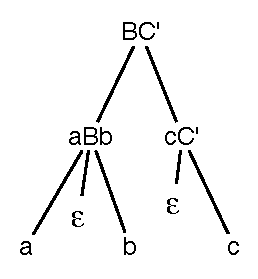
\includegraphics{problem_1_2_a.eps}
      }
      \subfigure[Tree 2]{
        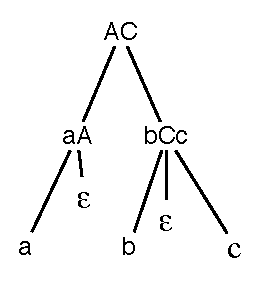
\includegraphics{problem_1_2_b.eps}
      }
    \end{figure}
  \end{solution}
\end{problem}

\begin{problem}{2}
\end{problem}

\begin{problem}{3}
  \begin{solution}
    We have a 6 tuple $<Q, \Sigma, \Gamma, \delta, q_1, F>$ \\
    \(
      Q = \{ q_1, q_2, \ldots, q_{11} \} \\
      \Sigma = \{ a, b \} \\
      \Gamma = \{R, S, T, X \} \cup \Sigma \\
      F = \{ Q_{11} \}
    \) \\
    And $\delta$ the transition function is represented by the figure below.
    \begin{figure}[H]
      \centering
      \caption{Transitions for PDF recognizing the grammar}
      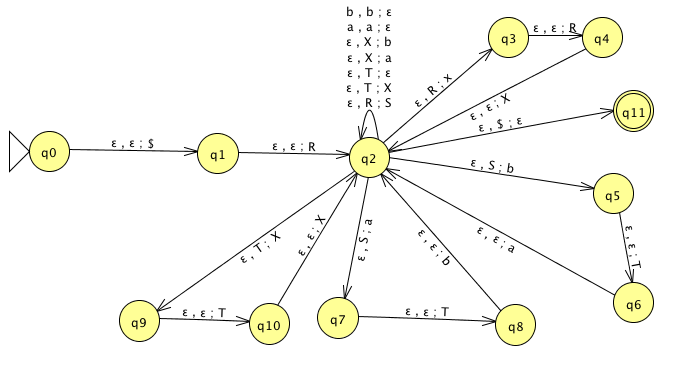
\includegraphics[scale=.6]{problem_3.png}
    \end{figure}
  \end{solution}
\end{problem}

\begin{problem}{4}
  Problem 2.14 from the book.
  \begin{solution}
    Step 1: Add a new start state $S_0$.
    \begin{align*}
      S_0 &\rightarrow A \\
      A &\rightarrow BAB|B|\epsilon \\
      B &\rightarrow 00|\epsilon
    \end{align*}
    Step 2: Remove epsilons.
    \begin{align*}
      S_0 &\rightarrow A | \epsilon \\
      A &\rightarrow BAB|B|A|AB|BA|BB \\
      B &\rightarrow 00
    \end{align*}
    Step 3: Remove unit rules.
    \begin{align*}
      S_0 &\rightarrow BAB|00|AB|BA|BB| \epsilon \\
      A &\rightarrow BAB|00|AB|BA|BB \\
      B &\rightarrow 00
    \end{align*}
    Step 4: Add additional rules.
    \begin{align*}
      S_0 &\rightarrow BD|CC|AB|BA|BB| \epsilon \\
      A &\rightarrow BD|CC|AB|BA|BB \\
      B &\rightarrow CC \\
      C &\rightarrow 0 \\
      D &\rightarrow AB
    \end{align*}
  \end{solution}
\end{problem}

\begin{problem}{5}
  Do Exercise 2.16 from the book.
  \begin{solution}
    Let $L_1 = <V_1, \Sigma, R_1, S_1>$ and $L_2 = <V_2, \Sigma, R_2, S_2>$. \\ We can prove each operation by
    constructing some CFG to recognize it generally.
    \br
    \textbf{First, union:} \\ $L_1 \cup L_2 = < V_1 \cup V_2 \cup \{S\}, \Sigma,
    R_1 \cup R_2 \cup \{ S \rightarrow S_1|S_2 \}, S \}$ where any conflicting variable names have been renamed.
    \br
    \textbf{Concatination:} \\
    $L_1 \circ L_2 = < V_1 \cup V_2 \cup \{S\}, \Sigma, R_1 \cup R_2 \cup \{ S \rightarrow S_1S_2 \}, S \}$
    where any conflicting variable names have been renamed.
    \br
    \textbf{Star:} \\
    $L_1^* = < V_1 \cup \{S\}, \Sigma, R_1 \cup \{ S \rightarrow SS_1|\epsilon \}, S \}$
  \end{solution}
\end{problem}

\begin{problem}{6}
  Do Exercise 2.2 from the book.
  \begin{solution}
    a. We can show a CFG trivially for A and B.
    \br
    A:
    \begin{align*}
      S &\rightarrow AB \\
      A &\rightarrow aA|\epsilon \\
      B &\rightarrow bBc|\epsilon
    \end{align*}
    B:
    \begin{align*}
      S &\rightarrow AC \\
      A &\rightarrow aAb|\epsilon \\
      C &\rightarrow cC|\epsilon
    \end{align*}
    The intersection is $A \cap B = \{ a^nb^nc^n|n \ge 0 \}$ but Example 2.36 shows by pumping lemma that $\{
    a^nb^nc^n|n \ge 0 \}$ is not context free. Since there is at least one intersection that isn't closed we can
    conclude that CFGs are not closed under intersection.
    \br
    b. We can show $A \cup B$ as:
    \begin{align*}
      S &\rightarrow AB|XC \\
      A &\rightarrow aA|\epsilon \\
      B &\rightarrow bBc|\epsilon \\
      X &\rightarrow aXb|\epsilon \\
      C &\rightarrow cC|\epsilon
    \end{align*}
    So this is a CFG for $A \cup B$. Assuming CFGs are closed under complementation we have $\overline{A} \cup \overline{B}$ is a CFG as well. But using DeMorgan's laws we have $\overline{\overline{A} \cup \overline{B}} \equiv A \cap B$ which was demonstrated in part A to not be a CFG. Therefore by contradiction CFGs are not closed under complementation. \qed
  \end{solution}
\end{problem}

\begin{problem}{7}
  \begin{solution}
    1. From Problem 2.18 part a we know $L \cap R$ is context free. $L - R = L \cap \overline{R}$ (see figure~\ref{fig:venn} below).
    Since the complement of R is also regular, and $L \cap R$ is context free, $L - R$ is context free. \qed
    \begin{figure}[H]
      \centering
      \caption{Venn Diagrams}
      \subfigure[Complement of R]{
        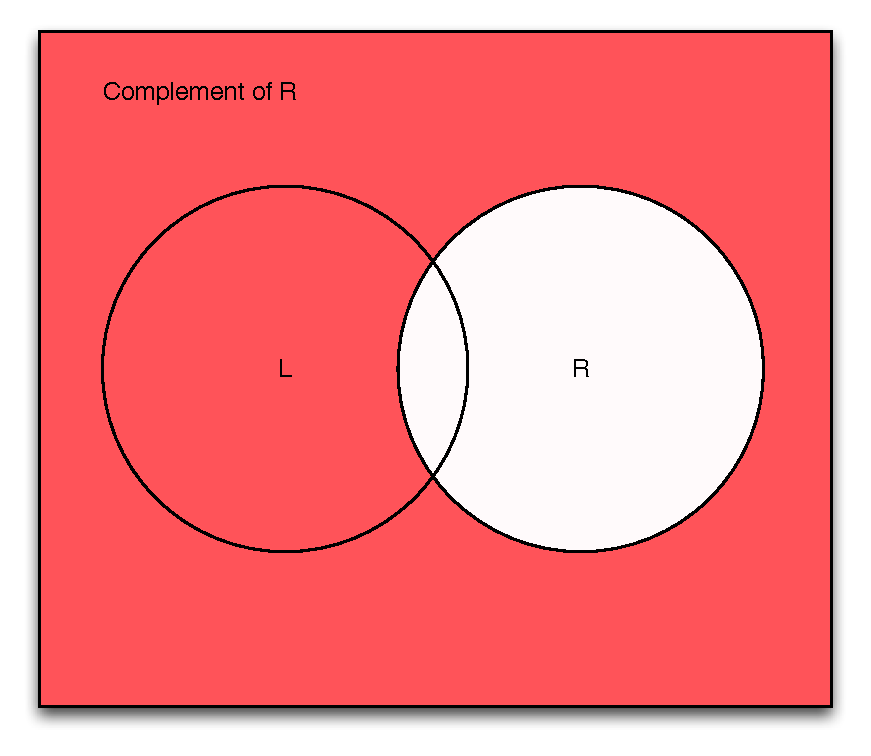
\includegraphics[scale=.4]{problem_7_a.eps}
      }
      \subfigure[L intersect R complement]{
        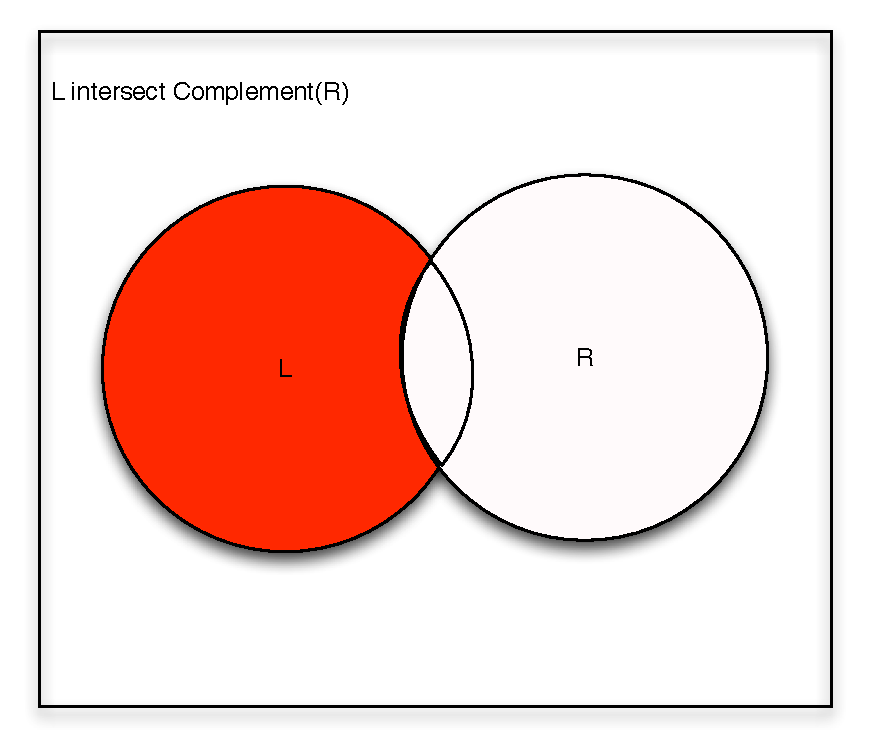
\includegraphics[scale=.4]{problem_7_b.eps}
      }
      \label{fig:venn}
    \end{figure}
    \noindent 2. If we try to do the same thing above, only this time with R - L, we would have to take the complement of L. But we proved in problem 6 that context free languages are not closed under complementation. Therefore we can't use the set property $R - L = R \cap \overline{L}$ because the complement of L may not be a context free language.
  \end{solution}
\end{problem}

\begin{problem}{8}
\end{problem}

\begin{problem}{9}
  Do Problem 2.44 from the book. Hint: Think of constructing a PDA for $A \Diamond B$ from the DFAs that are known to exist for A
  and B.
  \begin{solution}
    Let $DFA_A = \tuple{Q_A, \Sigma, \delta_A, q_A, F_A}$ recognize the language of A. \\
    Let $DFA_B = \tuple{Q_B, \Sigma, \delta_B, q_B, F_B}$ recognize the language of B. \\
    Let $M_{A \Diamond B} = \tuple{Q, \Sigma, \Gamma, \delta, q_0, \{ q_F \}}$ be some PDA recognizing $A \Diamond B$ where:
    \br
    $Q = Q_a \cup Q_b \cup \{ q_0, q_F \}$ \\
    $\Gamma = \{ \$, x \}$, \$ is the start of the stack and x counts symbols in A.
    \br
    \[
      \delta(q, a, b) =
      \begin{cases}
        \{ q_A, \$ \} &\text{ if } q = q_0 \text{ and } a = b = \epsilon \\
        \{ \delta_A(q, a), x\} &\text{ for all } q \in Q_a \text{ and } a \in \Sigma \text{ and } b = \epsilon \\
        \{ q_B, \epsilon \} &\text{ if } q \in Q_F \text{ and } a = b = \epsilon \\
        \{ \delta_B(q, a), \epsilon \} &\text{ for all } q \in Q_b \text{ and } a \in \Sigma \text{ and } b = x \\
        \{ q_F, \epsilon \} &\text{ if } q \in F_b \text{ and } b = \$ \text{ and } a = \epsilon \\
        \text{else } &\emptyset
      \end{cases}
    \]

  \end{solution}
    So the PDA pushes \$ onto the stack then transitions to the start state of $Q_A$. From there the PDA runs through
    the machine A, and for each symbol read by A it pushes $x$ onto the stack. From the accept states of A it
    transitions to B and then runs through B, this time popping an $x$ off the stack each symbol B reads. If B is in the
    accept state and the stack is empty denoted by \$ the PDA moves into its accept state.
\end{problem}

\end{document}
